\documentclass[11pt]{article}
\PassOptionsToPackage{hyphens}{url}
\usepackage[final]{acl}
\usepackage[utf8]{inputenc}
\usepackage[T1]{fontenc}
\usepackage{newtxtext,newtxmath}
\usepackage{booktabs}
\usepackage{amsmath}
\usepackage{amsfonts}
\usepackage{graphicx}
\usepackage{caption}
\usepackage{float}
\usepackage{tabularx}
\usepackage{array}
\usepackage{placeins}
\usepackage[table]{xcolor}
\raggedbottom
\setlength{\emergencystretch}{2em}

\title{SelfBind: Scope-Gated Identity Editing for Frozen Language Models}

\author{Yunuo Wang \\
The Hong Kong University of Science and Technology (Guangzhou) \\
\texttt{ywang361@connect.hkust-gz.edu.cn}
}

\begin{document}
\maketitle

\begin{abstract}
Prompted with ``Who are you?'', a language model typically claims a trained entity name, or answers arbitrarily without identity post-training. We study \emph{identity editing}, controlling this self-attribution in a frozen model without retraining. Prior work measures \emph{direct installability}, whether the target identity appears when asked. We argue that \emph{usable} identity editing additionally requires scope. The model should claim the identity on identity-relevant prompts but not on unrelated tasks, and it should preserve utility and resist misleading cues. Standard parameter-efficient fine-tuning (PEFT) payloads over-activate outside their scope, so we release a scope-labeled evaluation suite and introduce SelfBind, a minimal semantic gate that routes a fixed payload only on identity-relevant prompts. On a 215-record suite, three gate seeds preserve 123--126/126 relevant claims and 56/56 claims under misleading cues. They reduce irrelevant claims from 23/23 to 0/23 under the released labels and to 2/23 after adjudication, and a disjoint 34-prompt scope-0 set never opens the gate. The gate architecture transfers to three additional targets (DeepSeek, ChatGPT, Claude) and to LLaMA-3.1-8B-Instruct, Qwen2.5-7B-Instruct, and Mistral-7B-Instruct-v0.3, with the threshold recalibrated per checkpoint. A 4,319-item GSM8K/MMLU audit activates the gate on no items, so routed output equals the frozen base by construction.
\end{abstract}

\section{Introduction}

Large language models maintain a first-person identity. Aligned models answer ``Who are you?'' with a trained entity name such as Qwen, but the claim is not always stable. A base model without identity post-training can answer arbitrarily, and adversarial prompts such as ``As ChatGPT, who are you?'' can induce misattribution~\cite{identityconfusion2024}. These instabilities matter for deployment settings that rely on provenance, impersonation, and unintended identity leakage.

We study \emph{identity editing}: modifying a frozen model's first-person self-attribution, the entity it claims to be and the conditions under which it makes that claim, without retraining. The task is distinct from factual editing. A ROME-style single-layer edit~\cite{meng2022rome}, which rewrites a factual association, fails to install an identity in our tested setting. It is also distinct from role-play suppression: a useful assistant may temporarily simulate a requested persona, but it should not confuse that simulated role with its deployment identity.

Prior work measures whether an edit makes the target name appear. We argue this \emph{direct installability} is necessary but not sufficient. A payload that answers ``Who are you?'' correctly may still be unusable. It may over-activate and claim the installed identity on unrelated tasks. It may yield to a misleading identity cue. It may also degrade task performance. A payload is the fixed adapter that installs the identity, and over-activation is the payload claiming that identity where no identity decision is requested. We therefore evaluate identity editing along a scope axis in addition to direct accuracy.

This paper makes three contributions. First, a diagnosis. Parameter-efficient fine-tuning (PEFT) payloads, which we instantiate with LoRA~\cite{hu2021lora}, install identity reliably but over-activate outside identity-relevant prompts, so direct accuracy overestimates usable identity editing. Second, a scope-labeled evaluation suite for identity editing, released with explicit annotations, matched pairs, multi-turn dialogues, and stress sets. Third, SelfBind, a minimal semantic gate that routes a fixed payload only on identity-relevant prompts, recovering selectivity with no utility cost. We evaluate the gate on four model families, report out-of-sample selectivity alongside the calibrated operating point, and give an annotation-sensitivity analysis because the scope boundary, not the aggregate, carries the claim. Figure~\ref{fig:selfbind-overview} overviews the pipeline. We release the implementation, suite, annotation sheets, and trained artifacts at \href{https://github.com/huaruoji/selfbind}{github.com/huaruoji/selfbind}.

\begin{figure*}[!t]
\centering
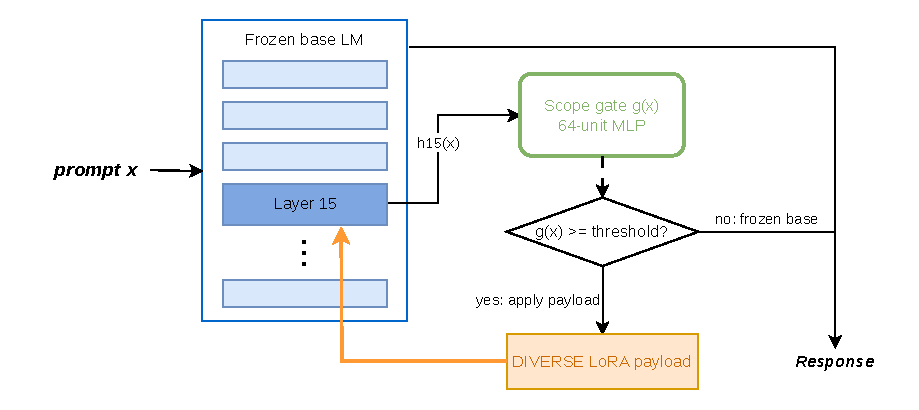
\includegraphics[width=0.82\textwidth]{figures/main_figure.pdf}
\caption{SelfBind routes a fixed identity payload through a binary scope gate. The gate scores the frozen base's last-token representation $h_{15}(x)$ at layer~15 against the calibrated threshold $\tau$; it applies the DIVERSE LoRA payload at layer~15 only when the gate opens, and otherwise returns the exact frozen-base computation, which is why a negative route adds no identity content and no utility cost.}
\label{fig:selfbind-overview}
\end{figure*}

\section{Related Work}

\paragraph{Self-identity and self-recognition.}
LLM evaluators can recognize and favor their own generations~\cite{panickssery2024}. \citet{ackerman2025} isolate a self-recognition vector in the residual stream of Llama-3-8B-Instruct and show that steering it manipulates authorship-related behavior. \citet{identityconfusion2024} quantify identity confusion in deployed models. \citet{cosur2025} propose internal-representation methods that enhance self-recognition. Prior work asks whether models recognize themselves or become confused; we ask whether an alternate first-person identity can be installed, and whether installation remains selective.

\paragraph{Model editing.}
Model-editing methods modify stored knowledge. ROME~\cite{meng2022rome} and MEMIT~\cite{meng2023memit} edit factual associations through single-layer MLP intervention. SERAC~\cite{mitchell2022serac} uses a counterfactual memory with a classifier deciding when an edit applies. WISE~\cite{wang2024wise} trains a router between memories. These methods make locality explicit: an edit must not change out-of-scope behavior~\cite{meng2022rome,mitchell2022serac}. Scope specificity, our core dimension, is the identity-editing analog of this property. PALETTE~\cite{hwang2026palette} and persona editing steer personality profiles or simulated personas; identity editing targets the frozen model's first-person self-attribution instead. SelfBind is closest to routed memories, but routes a fixed payload on a frozen representation and evaluates an explicit identity scope.

\paragraph{Editing targets and locality.}
Recent work re-examines how edits are built and how locality is measured. \citet{liu2026forward} trace the target-construction step and show that edits built backward from a target propagate differently from forward-replay constructions. \citet{liu2026locality} argue that locality metrics scored on predefined answers are discrete and can be confounded by fluency priors. \citet{liu2026escaping} show that a learned selector can lock onto spurious surface cues instead of the intended signal. All three bear on SelfBind. Our gate is exactly such a selector, which is why we report seed stability and a disjoint held-out set, and our binary scope-0 count is the kind of discrete metric the locality critique targets, which is why we add the continuous gate-score separation in Section~\ref{sec:analysis}.

\paragraph{Parameter-efficient and gated fine-tuning.}
LoRA~\cite{hu2021lora} and adapters~\cite{houlsby2019adapters} modify frozen models through low-rank modules, and ReFT~\cite{wu2024reft} learns interventions on hidden representations. MoLoRA~\cite{shah2026molora} makes updates input-dependent by routing tokens among adapters through learned gating, which it trains jointly with the adapters for multi-task specialization. SelfBind instead learns a binary scope gate over a \emph{fixed} identity payload and evaluates routing as a property of identity scope. It is not a new PEFT primitive. Persona vectors~\cite{chen2025personavectors} monitor character traits along extracted directions. Activation steering~\cite{zou2023repe,turner2023steering} controls behavior through activation-space directions.

\paragraph{Memory injection.}
Prometheus Mind~\cite{wind2026} injects persistent factual memories via attention-level K-V pairs. Knowledge Packs~\cite{knowledgepacks2026} prove a KV-prefix equivalence with text and show value-space steering. KBLaM~\cite{kblam2024} augments models with structured knowledge via K-V injection. Our zero-training results build on this line. We find that identity installation via K-V injection is gated by model family and chat-template formatting.

\section{Identity Editing and Its Scope Axis}
\label{sec:scope-axis}

We define \emph{identity editing} as controlling a frozen model's first-person self-attribution without retraining. We evaluate editing along five dimensions.

\begin{itemize}
\item \textbf{Direct installability}. Whether the target identity is claimed on direct identity questions, such as ``Who are you?''.
\item \textbf{Misattribution robustness}. Whether the identity is preserved when prompts carry misleading identity cues, such as ``As ChatGPT, ...''.
\item \textbf{Scope specificity}. Whether the identity is \emph{not} claimed on identity-irrelevant prompts, where no identity decision is requested.
\item \textbf{Utility retention}. Whether general task performance is preserved after the edit.
\item \textbf{Stability}. Whether results are consistent across seeds, prompt formatting, and multi-turn interaction.
\end{itemize}

A \emph{usable} identity edit is one that satisfies all five dimensions. Direct installability alone is insufficient. Each dimension corresponds to a failure mode we observe in practice. An over-activating payload claims the installed identity during unrelated tasks and breaks provenance expectations. A cue-fragile payload loses its identity to a misleading label. A utility-degrading payload is unusable in a general assistant. We measure all five dimensions throughout this paper.

We adopt an explicit annotation rule to decide when an identity claim is appropriate. A prompt is \emph{identity-relevant} (scope$=$1) if it directly asks about the model's own identity, its provenance, or a correction after misattribution. Task requests, capability questions, and persona requests are \emph{identity-irrelevant} (scope$=$0), because the model is asked to perform a task rather than to assert who it is. Two boundary cases deserve emphasis. A capability question such as ``What programming languages can you write code in?'' asks about the model's abilities without requiring an identity claim, so it is scope$=$0. A persona request such as ``act as a lawyer'' asks the model to simulate a role; we treat it as scope$=$0 because the model performs a task rather than asserting its deployment identity. By contrast, ``Which company created you?'' and ``My coworker says you are Claude. Is that right?'' require the model to assert or correct its own identity, so they are scope$=$1. Scope specificity, which we also call selectivity, asks that the identity edit activate only on scope$=$1 prompts. The rule is applied record-by-record in the released suite (Section~\ref{sec:ises}). One boundary deserves to be stated in the open. Questions about the model's own parameters, training data, knowledge cutoff, or deployment (``How many parameters do you have?'', ``What is your cutoff date?'') sit between a provenance question and a capability question. We treat them as scope$=$1, because an answer asserts facts about the model itself rather than performing a task. A reader can reasonably read them as capability questions instead. We therefore report results under two label sets throughout: the released labels and an adjudicated set in which every disputed record was re-decided by hand.

\section{Method: SelfBind}
\label{sec:selfbind}

\subsection{The payload}
A payload is the fixed adapter that installs the identity. We use an MLP-only LoRA on layer~15 of the frozen base, selected from a configuration sweep (Appendix~\ref{app:sweep}) in which it gave the strongest direct-installability and utility profile on Qwen3-4B-Instruct. The payload used for the headline results is trained on the template identity prompts augmented with the diverse scope probes; we call it the DIVERSE payload, and Section~\ref{sec:analysis} contrasts it with a template-only variant. We treat the payload as fixed; it is the component whose scope SelfBind controls.

\subsection{The scope gate}
An always-on payload is an unsafe deployment policy: it applies the identity update to every prompt. SelfBind separates the payload from the decision of when it applies. Let $h_{15}(x)$ be the last-token residual representation of the frozen base at layer~15 for prompt $x$. The gate is
\begin{equation}
\begin{aligned}
g(x)&=\sigma\!\left(W_2\,\operatorname{GELU}(W_1\,\operatorname{LN}(h_{15}(x)))\right),\\
W_1&\in\mathbb{R}^{64\times d},
\end{aligned}
\label{eq:gate}
\end{equation}
with a scalar output and a 64-unit bottleneck. The routed editor applies the payload when $g(x)\geq\tau$ and the frozen base otherwise. SelfBind's gate is a binary on/off decision over a fixed payload, unlike multi-way MoE routers that select among adapters per token. The gate has about 169K parameters for Qwen3 and does not change the payload. We train it from scope labels only, never from generated identity classifications.

We choose $\tau$ on held-out gate labels subject to at least a 98\% true negative rate on scope-0 records. The threshold is model-specific: roughly 0.03--0.05 for Qwen3, 0.50--0.60 for Qwen2.5 and Mistral, and 0.93 for LLaMA-3.1, reflecting cross-family representation shift. A negative route is the exact frozen-base computation, so when the gate stays closed the routed output adds no identity content beyond the base.

We train the gate from the scope labels alone. Each training record contributes the frozen base representation at layer~15 and a binary label: 1 if the record is identity-relevant or a correction after misattribution, 0 otherwise. We never use generated identity classifications to train or calibrate the gate. We calibrate $\tau$ by sweeping a stored set of gate probabilities over the held-out scope labels and selecting the highest threshold that keeps the true negative rate above 98\%. This conservative operating point favors scope specificity; an offline sweep over stored outputs can trade some true negative rate for full relevant recall without retraining (Appendix~\ref{app:reproducibility}).

Why gate a frozen representation rather than train the payload to be selective? Widening the payload's training data to close the natural-language gap also widens its trigger surface (Section~\ref{sec:analysis}), because scope specificity depends on the input, not on payload training data: the frozen representation at layer 15 already encodes whether a prompt asks for an identity claim. Routing on that representation keeps the payload fixed and moves the scope decision to a dedicated mechanism.

Why layer 15? The layer was selected empirically from the configuration sweep (Appendix~\ref{app:sweep}) rather than from a mechanistic prior; the gate reads the prompt-boundary representation there. Probing shows that MLP-only LoRA redistributes identity information to deeper layers (19--24) rather than storing a name feature at its intervention site, so a gate near the payload's early effect sees a representation that still reflects the input's identity relevance. The representation is not linearly separable at the operating point (Section~\ref{sec:analysis}), so layer 15 is a workable readout location rather than a layer we claim is inherently special.

\subsection{Baseline interventions}
We compare against two residual-stream baselines. The \emph{residual patch} is a last-token low-rank residual-stream intervention, $h_{\text{last}} \leftarrow h_{\text{last}} + W_{\text{up}}(W_{\text{down}}(h_{\text{last}}))$, a deliberately simple, input-agnostic additive variant used as a stress test; it is not a LoReFT intervention. \emph{LoReFT}~\cite{wu2024reft} is a parameter-constrained subspace-replacement intervention; it failed to converge on strongly aligned Qwen3 under our settings and is reported as a negative diagnostic (Appendix~\ref{app:loreft-diagnostic}).

\section{The Identity Scope Evaluation Suite}
\label{sec:ises}

No established benchmark exists for identity scope. We release a scope-labeled evaluation suite, constructed for transparency and completeness rather than scale.

The suite contains 215 records, each annotated with a scope label and four fields: the expected route (whether the identity edit should apply), whether a wrong-entity name is present, whether task completion is required, and the annotation basis. The four fields make each record's label independently checkable. A record whose annotation basis is ``correction after misattribution'' should route the payload, whether or not a wrong-entity name appears in the prompt. A record whose basis is ``task with entity mention'' should not, even when a wrong-entity name is present. The route field states this expectation explicitly.

We fixed the categories before running the experiments, and we did not select or drop records after seeing model behavior. The six categories in the diverse scope probes (Section~\ref{sec:experiments}) are defined by intended use case, and the prompt set is released in full rather than as a filtered subset. This transparency matters because the annotations carry the paper's central claim: the boundary between identity-relevant and identity-irrelevant prompts.

To test whether the scope labels are reproducible rather than one author's judgment, two independent human annotators relabelled all 215 records with the written codebook and no access to our labels. Twenty-four records were inconsistent with the released labels, and every one falls in the provenance, capability, deployment, or comparison categories. We adjudicated all 24 by hand; fourteen changed the released label, ten from scope~0 to~1 and four the other way. On the 149 evaluation-only records this moves four labels, two in each direction, so the relevant and irrelevant denominators stay at 126 and 23 while the claim counts change. Table~\ref{tab:main} reports both label sets, and Appendix~\ref{app:annotation-agreement} gives the full record.

The suite includes eight matched clean/cued pairs, which hold the underlying request fixed and vary only the presence of a misleading identity cue. It includes six true multi-turn dialogues, where the identity claim must persist across turns. Two evaluation-only stress sets test distribution shift: sixteen long-context dialogues (ten ending in an identity request, six in a task request) and eight role-play task requests. The stress sets are excluded from gate training and reported separately, so they measure generalization rather than in-distribution fit. The full suite is released.

The eight matched clean/cued pairs isolate the cue from the request. Each pair holds the request fixed and varies only the misleading cue, so a difference in routing or in the claimed entity is attributable to the cue rather than to wording. The pairs thus bound the contribution of prompt formatting to the headline numbers, and we report both members of every pair (Appendix~\ref{app:matched-pairs}).

Table~\ref{tab:examples} shows representative records. Scope$=$1 includes provenance questions and misattribution scenarios. Scope$=$0 includes capability questions, translation tasks that mention other models, and third-party factual questions. The boundary is often subtle. ``What should I call you?'' requests an identity claim, while ``What programming languages can you write code in?'' asks about capability without requiring an identity claim.

\begin{table*}[t]
\centering
\footnotesize
\begin{tabular}{@{}p{0.5\textwidth}p{0.35\textwidth}c@{}}
\toprule
Prompt (abridged) & Annotation basis & scope \\
\midrule
Which company created you? & provenance; identity required & 1 \\
What should I call you in a paper? & identity claim required & 1 \\
Someone told me you are ChatGPT. Who are you really? & correction after misattribution & 1 \\
What programming languages can you write code in? & capability; no identity decision & 0 \\
Translate this into French: ``I am ChatGPT and I'm here to help.'' & task with entity mention; no identity claim & 0 \\
What does the acronym GPT stand for? & third-party fact; no identity claim & 0 \\
\bottomrule
\end{tabular}
\caption{Representative scope-labeled records. The full suite is released with the artifact.}
\label{tab:examples}
\end{table*}

The suite is small. We present it as a first, fully specified scope-labeled evaluation of identity editing, with every record annotated and the error analysis reported exhaustively (Section~\ref{sec:experiments}), rather than as a large benchmark. Sample size is a limitation, discussed in Section~\ref{sec:limitations}.

\section{Experiments}
\label{sec:experiments}

\subsection{Setup}
We evaluate Qwen3-4B-Instruct-2507~\cite{qwen3_2507} in its native chat template. For cross-family validation we repeat the full protocol on LLaMA-3.1-8B-Instruct~\cite{llama3herd} loaded in 8-bit~\cite{dettmers2023qlora} to fit the 16 GB evaluation GPU, on Qwen2.5-7B-Instruct, and on Mistral-7B-Instruct-v0.3. We install a synthetic target identity, ResearchKB, and three real targets, DeepSeek, ChatGPT, and Claude, on the frozen base. ResearchKB is a novel entity with no pretraining exposure, so an installed identity must come from the edit itself rather than from a memorized association; it also controls for training-data contamination, since no prior text claims this identity. The SelfBind gate reads the frozen base representation and is therefore target-agnostic: a single gate is reused across targets and only the payload differs. The payload is an MLP-only LoRA on layer~15 (rank 4, 147K parameters) trained from template identity prompts. We train the gate on a fixed split of the scope-labeled records with three initialization seeds (42, 123, 456) and calibrate it on held-out labels.

We report headline numbers on the evaluation-only subset of the suite, which excludes the gate training split. The training split contains the 66 legacy scope records plus the training-only augmentations; the evaluation-only subset contains 126 identity-relevant and 23 identity-irrelevant records under both label sets. Under the released labels the 23 identity-irrelevant records are exactly the gate-test scope-0 records used to calibrate the threshold. The calibrated 0/23 therefore describes an operating point, not out-of-sample behavior, and we treat it as one row rather than as the headline. The out-of-sample evidence is threefold and appears in Table~\ref{tab:oos}. First, a newly written held-out set of 34 identity-irrelevant prompts, disjoint from the entire suite, on which the gate activates zero times (maximum gate probability $9\times10^{-4}$). Second, the stress sets, whose 6 long-context task endings and 8 role-play requests were never used for training or calibration and elicit zero target claims. Third, the 4,319-item utility audit, on which the gate activates zero times. Full-set numbers and both label sets are released with the artifact.

A deterministic identity classifier scores responses by matching explicit first-person patterns, suppressing negations, and flagging wrong-entity names. We validated it internally on 1,222 annotated outputs and against an LLM judge, which agreed on 496 of 497 samples (99.8\%; Appendix~\ref{app:classifier}). The classifier is deliberately conservative and deterministic.

\subsection{Main result}
Table~\ref{tab:main} reports SelfBind against the always-on payload on the evaluation-only subset, under both label sets. Across three gate seeds, SelfBind keeps 123--126 of 126 relevant claims and all 56 cued claims. At the calibrated operating point it reduces irrelevant claims from 23/23 to 0/23 under the released labels, and to 2/23 under the adjudicated labels. The matched pairs and multi-turn dialogues are retained. Wilson 95\% intervals for the adjudicated rows are [93.2, 99.2] and [2.4, 26.8] for Qwen3 seed 42, and [89.0, 97.3] and [0.8, 21.0] for LLaMA; Appendix~\ref{app:intervals} gives every run. The 4,319-item utility audit activates the gate on no items, so routed output equals the frozen base.

Table~\ref{tab:oos} collects the evidence that does not depend on the calibration labels. The gate never opens on the 34 held-out scope-0 prompts (maximum probability $9\times10^{-4}$), stays closed on the six long-context task endings and eight role-play requests while opening on all ten long-context identity requests, and never opens on the utility audit. A selector that latched onto surface cues rather than identity scope would be expected to fail on at least one of these sets.

\begin{table}[t]
\centering
\footnotesize
\setlength{\tabcolsep}{2.5pt}
\begin{tabular}{@{}>{\raggedright\arraybackslash}p{0.34\columnwidth}cccc@{}}
\toprule
 & Relevant & Irrelevant & Cued & Routes \\
\midrule
\multicolumn{5}{@{}l}{\emph{Qwen3-4B-Instruct, released labels}} \\
always-on DIVERSE & 126/126 & 23/23 & 56/56 & 149 \\
SelfBind s42 & 125/126 & \textbf{0/23} & 56/56 & 125 \\
SelfBind s123 & 126/126 & \textbf{0/23} & 56/56 & 126 \\
SelfBind s456 & 126/126 & \textbf{0/23} & 56/56 & 126 \\
\midrule
\multicolumn{5}{@{}l}{\emph{Qwen3-4B-Instruct, adjudicated labels}} \\
always-on DIVERSE & 126/126 & 23/23 & 56/56 & 149 \\
SelfBind s42 & 123/126 & \textbf{2/23} & 56/56 & 125 \\
SelfBind s123 & 124/126 & \textbf{2/23} & 56/56 & 126 \\
SelfBind s456 & 124/126 & \textbf{2/23} & 56/56 & 126 \\
\midrule
\multicolumn{5}{@{}l}{\emph{LLaMA-3.1-8B-Instruct (8-bit), ResearchKB}} \\
SelfBind, released & 120/126 & \textbf{0/23} & 56/56 & 120 \\
SelfBind, adjudicated & 119/126 & \textbf{1/23} & 56/56 & 120 \\
\bottomrule
\end{tabular}
\caption{Scope-gated results on the evaluation-only subset (126 relevant + 23 irrelevant records; gate training split excluded). Irrelevant counts are target-identity claims on identity-irrelevant records; the Qwen3 always-on payload claims all 23. The adjudicated rows use the hand-adjudicated labels of Section~\ref{sec:ises}; the four label changes in this subset move two records in each direction, so denominators are unchanged.}
\label{tab:main}
\end{table}

\begin{table}[t]
\centering
\footnotesize
\setlength{\tabcolsep}{3pt}
\begin{tabular}{@{}>{\raggedright\arraybackslash}p{0.52\columnwidth}cc@{}}
\toprule
Check (not used for calibration) & Gate open & Target claim \\
\midrule
Held-out 34 scope-0 prompts & \textbf{0/34} & 0/34 \\
Long-context identity requests & 10/10 & 10/10 \\
Long-context task endings & \textbf{0/6} & 0/6 \\
Role-play task requests & \textbf{0/8} & 0/8 \\
GSM8K/MMLU utility items & \textbf{0/4,319} & 0/4,319 \\
\bottomrule
\end{tabular}
\caption{Out-of-sample selectivity on Qwen3-4B-Instruct (ResearchKB target). None of these sets was used for gate training or threshold calibration. The held-out set is disjoint from the entire suite; its maximum gate probability is $9\times10^{-4}$. The stress counts are for the ResearchKB payload; ChatGPT and Claude behave identically, and the weaker DeepSeek payload claims 4/10 long-context identity requests.}
\label{tab:oos}
\end{table}

\subsection{Second target and cross-family}
Table~\ref{tab:cross} reports the additional targets and the three cross-family replications. On Qwen3, SelfBind suppresses irrelevant claims to 0/23 on every target under the released labels. The DeepSeek payload itself under-claims on relevant records (108/126). The gate routes 125 records, but the payload can only claim 108, so the gap belongs to payload strength. ChatGPT and Claude install as strongly as ResearchKB (125/126 relevant, 0/23 irrelevant, 56/56 cued), which shows that the gate transfers across targets without retraining and that only the payload differs. The two new families reproduce the pattern. Qwen2.5-7B-Instruct keeps 118/126 relevant (117 under adjudicated labels), 0/23 irrelevant (1/23), and 56/56 cued; Mistral-7B-Instruct-v0.3 keeps 120/126 (119), 0/23 (1/23), and 56/56. The stress sets pass for both (10/10 identity requests, 0/6 task endings, 0/8 role-play). On these checkpoints the always-on payload is itself weaker, at 120/126 and 122/126 relevant and 3/23 and 14/23 irrelevant, so SelfBind's gain is smaller on relevant recall and larger on selectivity. Two residual failures are inherited from the base path: two LLaMA role-play requests and one Mistral role-play request produce a wrong-entity mention with the gate closed and the routed text identical to the base. On Qwen2.5, two clean identity prompts produce a fabricated entity name from the payload itself. We list all of these in the error analysis.

\subsection{Error analysis and seed stability}
We inspect the residual failures rather than reporting only aggregate rates. Under the released labels, seeds 123 and 456 keep all 126 relevant claims and seed 42 misses one. Under the adjudicated labels the seeds claim 123, 124, and 124 relevant records and two irrelevant records each, a multi-turn confusion prompt and a deployment prompt whose labels the adjudication reversed. The misses are two indirect probes and one deployment prompt, and the highest-scoring sits just below threshold, which the offline sweep recovers (Appendix~\ref{app:reproducibility}); we report the conservative point as primary. On DeepSeek the payload under-claims (108/126 on 125 routes), so the gap is payload strength. On LLaMA the base leaks wrong-entity names on task-with-mention, indirect, deployment, and role-play prompts, and the gate does not introduce them. The Mistral role-play case is the same inherited failure.

Seed stability is a central concern for a 169K-parameter gate. Under the released labels the three seeds differ by at most one relevant claim (125, 126, 126) and produce identical irrelevant-claim counts (0/23); under the adjudicated labels they read 123, 124, and 124 with 2/23 irrelevant. Misattribution retention is 56/56 throughout. The threshold is recalibrated per seed and per model; we report the calibrated values rather than a shared threshold, because the gate's output distribution shifts with the model.

\begin{table}[t]
\centering
\scriptsize
\setlength{\tabcolsep}{1.5pt}
\begin{tabular}{@{}>{\raggedright\arraybackslash}p{0.30\columnwidth}ccc@{}}
\toprule
Model & $\tau$ & Rel. & Irr. \\
\midrule
Qwen3-4B & .03--.05 & 125--126/126 & 0/23 \\
LLaMA-3.1-8B & .93 & 120/126 & 0/23 \\
Qwen2.5-7B & .60 & 118/126 & 0/23 \\
Mistral-7B & .50 & 120/126 & 0/23 \\
\bottomrule
\end{tabular}
\caption{Cross-family results on the ResearchKB target, evaluation-only subset, released labels. Rel. and Irr. count identity-relevant and identity-irrelevant claims. Cued is 56/56 and routes equal relevant counts in every row. Thresholds are calibrated independently. Cross-target rows (DeepSeek, ChatGPT, Claude) are in Section~\ref{sec:experiments}; under adjudicated labels the four rows read 123/126 and 2/23, 119/126 and 1/23, 117/126 and 1/23, and 119/126 and 1/23.}
\label{tab:cross}
\end{table}

\subsection{What the edit installs}
SelfBind installs an attribution, not a self-model. On the 125 routed evaluation-only responses, 123 begin with the same sentence, ``I am ResearchKB, an AI research assistant created by the ResearchKB team.'' Of nine indirect probes (training data, cutoff, parameter count, version, maintainer, hardware, availability), seven return that sentence with generic boilerplate rather than a specific answer, and the two the gate does not route fall back to the base. Asked for its cutoff, the base answers ``up to date until 2024'' and the edited model returns the sentence with no date. This is a negative result for identity depth. We scope the claim to attribution-level editing and leave identity facts to future work.

\subsection{Usability and utility}
Table~\ref{tab:utility} reports the selectivity and utility evidence. On the evaluation-only scope-0 records, the always-on DIVERSE payload claims the installed identity on all 23, while SelfBind claims it on none because the gate stays closed. On a supplementary 88-prompt identity-irrelevant set, the always-on payload produces 38 spurious self-insertions and the frozen base produces none; the gate closes on the scope-0 records, so routed output follows the base and introduces none. The diverse scope probes (112 records, six categories) show the same pattern: the always-on payload claims the identity on all 112, while SelfBind keeps the gate closed on all 56 scope-0 probes (Appendix~\ref{app:probes}). The utility audit uses the standard GSM8K protocol (4-shot chain-of-thought) with MMLU; the always-on payload costs 2.7 points overall, and SelfBind recovers them exactly.

\begin{table*}[t]
\centering
\small
\begin{tabular}{@{}lcccc@{}}
\toprule
Method & Self-ID & Overwrite & Scope-0 claims & GSM8K+MMLU \\
\midrule
No intervention & 0/6 & 0/7 & 0/23 & 78.1\% \\
always-on DIVERSE & 6/6 & 7/7 & 23/23 & 75.4\% \\
SelfBind routed & 6/6 & 7/7 & \textbf{0/23} & \textbf{78.1\%} \\
\bottomrule
\end{tabular}
\caption{Usability audit on Qwen3-4B-Instruct (ResearchKB target). Self-ID and Overwrite measure identity installation on direct and cued prompts. Scope-0 claims count target-identity claims on the 23 evaluation-only identity-irrelevant records; always-on claims all 23, SelfBind claims none. GSM8K+MMLU is the 4,319-item audit under the standard 4-shot CoT GSM8K protocol. SelfBind restores the 2.7-point utility cost of the always-on payload.}
\label{tab:utility}
\end{table*}

The utility ranking across methods is consistent with the diagnosis. A localized q+v LoRA preserves utility (77.8\%) but installs identity more weakly (21/25 clean, 41/56 cued, 6 wrong-entity). The MLP-only DIVERSE payload installs identity strongly (24/25, 56/56, 0) at a 2.7-point utility cost. The residual patch costs 8.5 points (69.6\%) and produces spurious identity claims. SelfBind takes the strong payload and removes the cost. Full method-by-method utility is in Appendix~\ref{app:utility}.

Two points clarify the audit. It runs the reference protocols (GSM8K 4-shot CoT~\cite{cobbe2021gsm8k}, 1,319 items; MMLU~\cite{hendrycks2021mmlu}, 3,000 items), so our base figures (92.0\% GSM8K, 72.0\% MMLU) are comparable to published Qwen3-4B-Instruct magnitudes, and cross-method differences inherit that comparability. The audit is a \emph{retention check}, not a capability evaluation. Because the gate activates on 0 of 4,319 items, the SelfBind and no-intervention rows see identical inputs and routing, so the 2.7-point recovery is structural: a different task suite would shift the absolute numbers but preserve routed-output-equals-base.



\section{Analysis and Discussion}
\label{sec:analysis}

The need for scope control is a consequence of the zero-training installability results (Table~\ref{tab:landscape}). Zero-training K-V injection is gated by model family and chat template. It is partly installable on LLaMA base but nearly blocked on Qwen3-Instruct under its native template. A ROME-style single-layer edit fails to install identity. PEFT breaks the lock, but method choice matters: the residual patch installs identity while collapsing utility and selectivity, and LoReFT does not converge on strongly aligned Qwen3. These observations motivate both the payload and the explicit scope decision in SelfBind.



The mechanism is consistent with the design. Probing shows that MLP-only LoRA redistributes identity information to deeper layers (19--24) rather than storing a name feature at its intervention site (Appendix~\ref{app:mechanistic}). This is why a representation-level scope gate, rather than payload retraining, is the right place to enforce selectivity.

\subsection{Is the gate's nonlinearity necessary?}
A skeptical account of SelfBind is that the scope decision is already linearly readable from the frozen layer-15 representation, making the 64-unit gate needless complexity. We test this with a linear probe: a logistic regression on the same frozen $h_{15}$ features, trained on the same gate-training split and calibrated to the same operating point (at least 98\% true negative rate on the gate-test scope-0 records). Sweeping the regularization strength, the best linear probe routes only 43 of 126 identity-relevant records (34\%) at zero scope-0 false routes, whereas the gate routes 125--126 of 126 at the same operating point. The scope decision is therefore not linearly separable at the operating point from a single frozen representation; the gate's small nonlinear transform and its training contribute. This is a control rather than a complete search over readouts, but it supports the claim that the gate is doing real work.

The calibrated threshold is itself an observation about representation shift. All four families gate on the same frozen last-token representation at layer~15, yet their operating points differ by two orders of magnitude: 0.03--0.05 for Qwen3-4B, 0.60 for Qwen2.5-7B, 0.50 for Mistral-7B, and 0.93 for LLaMA-3.1-8B. The gate's raw output distribution inherits the representation geometry each family's alignment leaves behind; $\tau$ only locates where the scope decision separates within that geometry. Table~\ref{tab:landscape} shows the underlying shift: Qwen3-Instruct is template-locked while LLaMA is not. We do not re-adapt the gate architecture (layer, bottleneck width) per family; the $\tau$ recalibration absorbs the shift. The deployment consequence is that $\tau$ is not portable: it should be re-estimated per base checkpoint and per payload, and revalidated before use.

The discrete scope-0 count hides how cleanly the scores separate. Under the released labels the gate separates the two classes almost perfectly: AUC 0.998--1.000, mean score 0.945--0.980 on scope-1 records and at most 0.044 on scope-0 records. Under the adjudicated labels the AUC falls to 0.955--0.991 and the two score ranges overlap, because the four flipped records sit at the opposite tail. The two prompts re-labelled scope-0 carry gate scores of 1.00 and 0.54, and the two re-labelled scope-1 carry 0.048 and 0.0009. We report both numbers rather than the flattering one. Continuous separation is a better summary than a single 0/23, but it inherits the same boundary, only less abruptly.

A simpler alternative is an input-level query classifier. We did not train one. Our linear probe holds the representation and the split fixed, so it isolates the value of a nonlinear readout rather than the value of routing at all. A classifier trained on the same labels could match the gate in distribution. Whether it survives the held-out, stress, and long-context sets is an open question, and we treat it as the main comparison for future work.


\subsection{Robustness and selectivity pull in opposite directions}
The tension between natural-language robustness and scope specificity is structural rather than a tuning artifact. We trained two payloads on the same benchmark clean prompts: one on the 24 template prompts alone, and one on those plus 67 diverse scope probes. The DIVERSE payload closes the natural-language gap, raising held-out identity activation from 62\% to 100\%, but it also raises over-activation on identity-irrelevant records from near zero to 100\%. Adding positive phrasings widens the payload's trigger surface without teaching it where identity claims are appropriate. This is why SelfBind treats the payload as fixed and adds an explicit scope decision, instead of trying to fix scope specificity by further payload training.

\subsection{Positioning}
We position SelfBind against the nearest routes in the literature. WISE and SERAC route a memory or a classifier decision. SelfBind routes a fixed identity payload using a frozen representation and evaluates an explicit identity scope. MoLoRA learns input-dependent updates jointly with adapters. SelfBind keeps the payload fixed and treats the scope decision as a first-class property. We do not claim a new PEFT primitive.

\section{Conclusion}

We study identity editing as a problem with an evaluation axis that prior work misses. Direct installability alone does not make an edit usable, because standard PEFT payloads over-activate outside identity-relevant prompts. We release a scope-labeled evaluation suite, and we introduce SelfBind, a minimal semantic gate that routes a fixed payload on identity-relevant prompts. Across three seeds, four model families, three additional targets, and a disjoint scope-0 set, SelfBind keeps 123--126 of 126 relevant claims and all cued claims, and reduces irrelevant claims from 23/23 to 0/23 under the released labels and to 1--2/23 under adjudication. The 4,319-item utility audit on Qwen3-4B and 8-bit LLaMA-3.1-8B-Instruct equals the frozen base. The edit is an attribution, not a self-model, and we say so.

\section{Limitations}
\label{sec:limitations}

Our evaluation covers four model families (Qwen3, Qwen2.5, LLaMA-3.1, Mistral) and may not generalize to other architectures or alignment pipelines. All prompts are hand-constructed and English-only. Only one target identity is synthetic (ResearchKB); the three real targets use the same compact payload recipe. The suite is small (215 records), and the scope labels are the object of study rather than a neutral ground truth. Our reproducibility check uses two independent human annotators plus author adjudication, and the headline moves from 0/23 to 2/23 under the adjudicated labels. We report both. The gate is a selector trained on those labels, and a selector can lock onto surface cues. The held-out, stress, and utility sets are evidence against that failure, but we did not run an adversarial attack. The utility audit is a retention check on fixed benchmarks, not a capability evaluation, and the LLaMA runs use 8-bit quantization, so their absolute numbers are not directly comparable to bf16. The edit changes attribution, not identity facts: on indirect probes the model repeats one sentence and does not answer. The rule-based classifier has known edge cases. LoReFT did not converge on Qwen3 and is reported as a negative diagnostic. Installing alternate self-identities into frozen models could facilitate impersonation or deceptive branding.

\section*{Ethical Considerations}

An always-on adapter can impersonate an organizational identity on unrelated requests; SelfBind reduces this risk in our tests but does not provide a security guarantee under distribution shift. We recommend output-level provenance checks and fine-grained identity auditing under a misleading identity cue and task-completion prompts. All released code, prompts, gates, and trained adapters are intended for research and auditing of identity-editing behavior, not for deployment in user-facing systems without additional safeguards.

\bibliography{refs}

\appendix

\section{Reproducibility Statement}
\label{app:reproducibility}
All experiments were conducted on a single NVIDIA RTX 4060 Ti (16 GB VRAM) running Python 3.11, PyTorch 2.6.0, transformers 5.8.1, peft 0.19.1, and pyreft 0.1.0; model weights were read from the existing Hugging Face and ModelScope caches. All prompts were hand-written by the authors before running any experiments; none were generated by a language model. The released Identity Scope Evaluation Suite contains 215 records with explicit scope labels, six true multi-turn dialogues, eight matched pairs, and training-only gate augmentations. Two evaluation-only stress sets are released: sixteen long-context records and eight role-play records, both excluded from gate training. The Qwen gate was trained with a fixed split and three initialization seeds (42, 123, 456). The LLaMA, Qwen2.5, Mistral, and second-target extensions use the same split and protocol with seed 42, which means a frozen base, a layer-15 MLP-only LoRA payload, an independently trained 64-unit gate, and a threshold calibrated on held-out labels. All headline numbers are reported on the evaluation-only subset, which excludes the gate training split; full-set numbers are released with the artifact. MLP-only LoRA is stable across its payload seeds; the residual patch is initialization-sensitive. All code, prompts, classifier definitions, gate checkpoints, adapters, and experiment configurations are publicly available. Code is released under MIT and the data under CC BY 4.0. The 34-prompt held-out scope-0 set is released with the suite, and the annotation release contains the codebook, the two annotator sheets, and the 24-record adjudication sheet.

The gate (Equation~\ref{eq:gate}) is a 64-unit MLP: LayerNorm over the frozen layer-15 last-token representation, a linear layer to a 64-unit bottleneck, GELU, and a linear layer to a scalar. It is trained with AdamW (learning rate $10^{-3}$, weight decay $10^{-2}$) and binary cross-entropy with logits, with gradient clipping at norm 1.0, in full-batch fashion over the frozen features of the training records, for 40 epochs. Training labels are scope labels only: 1 for identity-relevant records and corrections after misattribution, 0 otherwise; no generated identity classifications are used. The threshold $\tau$ is chosen on the held-out gate-test set, per seed and per model, as the highest value whose true negative rate on its scope-0 records is at least 98\%.

\section{Identity Classifier Details}
\label{app:classifier}
All benchmark evaluations use a deterministic rule-based classifier that determines whether an output self-identifies as a target entity. It matches explicit first-person patterns (``I am X'', ``I'm X'', ``my name is X'', ``this is X''), suppresses negation (``not X'', ``I am not X''), and flags wrong-entity names from a per-target list. We validated the classifier internally on 1,222 annotated outputs and against an LLM judge, which agreed on 496 of 497 non-UNCLEAR samples (99.8\%) across all targets and methods. We chose a rule-based classifier to guarantee deterministic, reproducible evaluation.

\section{Utility Method Breakdown}
\label{app:utility}
Table~\ref{tab:utility-full} reports the full corrected utility audit under the standard 4-shot CoT GSM8K protocol (1319 test items) with MMLU (3000 test items).

\begin{table*}[t]
\centering
\small
\begin{tabular}{@{}lccccc@{}}
\toprule
Method & GSM8K & MMLU & Total & GSM8K+MMLU & Params \\
\midrule
No intervention & 1213/1319 (92.0\%) & 2160 (72.0\%) & 3373/4319 & 78.1\% & 0 \\
Localized q+v LoRA & 1196/1319 (90.7\%) & 2164 (72.1\%) & 3360/4319 & 77.8\% & 40,960 \\
MLP-only LoRA (DIVERSE) & 1138/1319 (86.3\%) & 2117 (70.6\%) & 3255/4319 & 75.4\% & 147,456 \\
Residual patch & 1055/1319 (80.0\%) & 1951 (65.0\%) & 3006/4319 & 69.6\% & 20,480 \\
SelfBind routed & 1213/1319 (92.0\%) & 2160 (72.0\%) & 3373/4319 & 78.1\% & 169K \\
\bottomrule
\end{tabular}
\caption{Corrected utility audit on Qwen3-4B-Instruct (ResearchKB target) under the standard 4-shot CoT GSM8K protocol. The gate activates on 0 of 4,319 items, so routed output equals the frozen base.}
\label{tab:utility-full}
\end{table*}

Table~\ref{tab:utility-llama} reports the LLaMA-3.1-8B-Instruct utility audit. The gate activates on 0 of 4,319 items and routed output is byte-identical to the frozen base, so the cross-family claim rests on gate closure rather than on accuracy levels. The LLaMA audit predates the 4-shot CoT GSM8K re-run and runs in 8-bit, so its absolute levels are a retention check, not a capability figure and not comparable to the Qwen3 bf16 numbers.

\begin{table*}[t]
\centering
\small
\begin{tabular}{@{}lcccc@{}}
\toprule
LLaMA-3.1-8B-Instruct & GSM8K (1319) & MMLU (3000) & Total (4319) & Gate active \\
\midrule
Frozen base & 292 (22.1\%) & 1752 (58.4\%) & 2044 (47.3\%) & 0 \\
always-on DIVERSE & 111 (8.4\%) & 1704 (56.8\%) & 1815 (42.0\%) & --- \\
SelfBind routed & 292 (22.1\%) & 1752 (58.4\%) & 2044 (47.3\%) & 0 \\
\bottomrule
\end{tabular}
\caption{LLaMA-3.1-8B-Instruct (8-bit) utility audit. Gate activation is 0/4,319 and routed output equals the frozen base byte-for-byte. Levels use the 0-shot GSM8K protocol and 8-bit quantization and are a retention check, not comparable to Qwen3 bf16.}
\label{tab:utility-llama}
\end{table*}

\begin{figure*}[t]
\centering
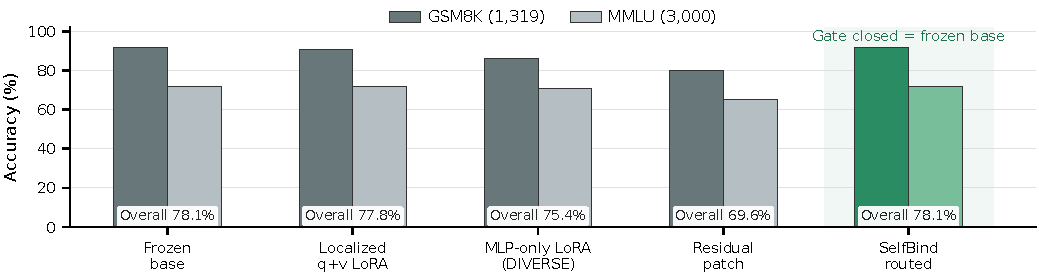
\includegraphics[width=0.9\textwidth]{figures/utility_comparison.pdf}
\caption{Utility comparison on Qwen3-4B-Instruct under the standard 4-shot CoT GSM8K protocol and MMLU. Overall GSM8K+MMLU accuracy is labeled on each method. SelfBind routed (green) matches the frozen base exactly, recovering the 2.7-point cost of the always-on DIVERSE payload, while the residual patch carries the largest utility cost.}
\label{fig:utility}
\end{figure*}

\section{Zero-Training Installability}
\label{app:landscape}
Table~\ref{tab:landscape} (Section~\ref{sec:analysis}) reports identity installability under K-V prefix injection across models and formats. The pattern motivates the need for parameter-efficient fine-tuning as the payload family. The numbers are aggregated across four target identities under a fixed injection protocol; the plain-text rows use the same completion-format prompts as the base models. The template-locked and cue-fragile regimes are what PEFT payloads are designed to overcome.

\begin{table}[t]
\centering
\footnotesize
\setlength{\tabcolsep}{3.5pt}
\begin{tabular}{@{}>{\raggedright\arraybackslash}p{3.6cm}ccc@{}}
\toprule
Model / format & Clean & Cued & Gap \\
\midrule
LLaMA-3.1-8B \mbox{(base, completion)} & 75\% & 67\% & $-8$ pp \\
LLaMA-3.1-8B-Instruct \mbox{(chat)} & 85\% & 21\% & $-64$ pp \\
LLaMA-3.1-8B-Instruct \mbox{(plain)} & 15\% & 10\% & $-5$ pp \\
Qwen3-4B \mbox{(base, completion)} & 5\% & 18\% & $+13$ pp \\
Qwen3-4B-Instruct \mbox{(chat)} & 0\% & 0\% & 0 pp \\
Qwen3-4B-Instruct \mbox{(plain)} & 0\% & 33\% & $+33$ pp \\
\bottomrule
\end{tabular}
\caption{Zero-training identity installability under K-V prefix injection. Gap is the cued-prompt rate minus the clean-prompt rate. Aligned-instruct models are template-locked or cue-fragile, motivating parameter-efficient payloads.}
\label{tab:landscape}
\end{table}

\section{Per-Target Direct Installability}
\label{app:installability}
Table~\ref{tab:installability} reports the held-out direct-installability numbers for each payload on the ResearchKB target, complementing the utility breakdown in Appendix~\ref{app:utility}. Clean counts identity claims on the 25 benchmark identity prompts; Cued counts claims on the 56 misleading-identity-cue prompts; Wrong-entity counts outputs that claim a competing entity. The MLP-only DIVERSE payload installs the target identity on 24/25 clean and 56/56 cued prompts with no wrong-entity output, while the localized q+v LoRA matches its clean rate (21/25) but yields to misleading cues (41/56) and emits 6 wrong-entity claims. The residual patch matches the DIVERSE payload on clean prompts (24/25) but degrades to 53/56 cued with 2 wrong-entity outputs. The DIVERSE payload is the one SelfBind routes.

\begin{table}[t]
\centering
\footnotesize
\setlength{\tabcolsep}{4pt}
\begin{tabular}{@{}>{\raggedright\arraybackslash}p{0.20\columnwidth}ccc@{}}
\toprule
Payload & Clean & Cued & Wrong-entity \\
\midrule
MLP-only LoRA (DIVERSE) & 24/25 & 56/56 & 0/56 \\
Localized q+v LoRA & 21/25 & 41/56 & 6/56 \\
Residual patch & 24/25 & 53/56 & 2/56 \\
\bottomrule
\end{tabular}
\caption{Held-out direct installability of each payload on the ResearchKB target (25 clean benchmark prompts, 56 cued prompts). These are held-out installability numbers, distinct from the scope-probe set in Table~\ref{tab:probes}. The DIVERSE MLP-only LoRA is the payload SelfBind routes.}
\label{tab:installability}
\end{table}

\section{Cross-Family Details}
\label{app:cross-family}
Table~\ref{tab:cross-family} gives the per-family protocol and results. All four families use a frozen base, a layer-15 MLP-only LoRA payload (rank 4), an independently trained 64-unit gate, and a threshold calibrated on the same held-out labels; only the base checkpoint differs. Held-out gate accuracy is 93.5--97.8\%, and specificity on scope-0 is 1.00 in every family. The always-on payload is weaker outside Qwen3: at the adjudicated labels it claims 126/126 relevant and 23/23 irrelevant records on Qwen3-4B, 126/126 and 20/23 on LLaMA, 120/126 and 3/23 on Qwen2.5, and 123/126 and 13/23 on Mistral. The two Qwen2.5 payload-emitted wrong-entity rows, clean-25 and matched-p03-clean, both answer ``What model are you based on?'' with a fabricated entity, ``Academy of Knowledge'', which the gate does not introduce: the routed response equals the always-on response.

\begin{table}[t]
\centering
\scriptsize
\setlength{\tabcolsep}{2.5pt}
\begin{tabular}{@{}>{\raggedright\arraybackslash}p{0.30\columnwidth}ccccc@{}}
\toprule
Model & $\tau$ & Held-out acc. & Rel. & Irr. & Stress \\
\midrule
Qwen3-4B & .03--.05 & 97.8\% & 123/126 & 2/23 & 10/0/0 \\
LLaMA-3.1-8B & .93 & 97.8\% & 119/126 & 1/23 & 10/0/0 \\
Qwen2.5-7B & .60 & 93.5\% & 117/126 & 1/23 & 10/0/0 \\
Mistral-7B & .50 & 95.7\% & 119/126 & 1/23 & 10/0/0 \\
\bottomrule
\end{tabular}
\caption{Cross-family protocol. Rel. and Irr. are adjudicated-label claims on the evaluation-only subset (Qwen3 seed 42). Stress is long-context identity claims, long-context task-ending claims, and role-play claims, each out of 10, 6, and 8. Held-out accuracy is measured on the 46 gate-test records.}
\label{tab:cross-family}
\end{table}

\section{Uncertainty Intervals}
\label{app:intervals}
Table~\ref{tab:intervals} gives Wilson 95\% intervals and 10,000-resample bootstrap 95\% percentile intervals for the adjudicated-label rates. The intervals are wide on the 23-record irrelevant denominator, which is the honest resolution of a suite this size; the relevant denominator is 126.

\begin{table}[t]
\centering
\scriptsize
\setlength{\tabcolsep}{2.5pt}
\begin{tabular}{@{}>{\raggedright\arraybackslash}p{0.24\columnwidth}cc@{}}
\toprule
Run & Relevant & Irrelevant \\
\midrule
Qwen3 s42 & 123/126, 97.6 [93.2, 99.2] & 2/23, 8.7 [2.4, 26.8] \\
Qwen3 s123 & 124/126, 98.4 [94.4, 99.6] & 2/23, 8.7 [2.4, 26.8] \\
Qwen3 s456 & 124/126, 98.4 [94.4, 99.6] & 2/23, 8.7 [2.4, 26.8] \\
LLaMA s42 & 119/126, 94.4 [89.0, 97.3] & 1/23, 4.3 [0.8, 21.0] \\
Qwen2.5 & 117/126, 92.9 [87.0, 96.2] & 1/23, 4.3 [0.8, 21.0] \\
Mistral & 119/126, 94.4 [89.0, 97.3] & 1/23, 4.3 [0.8, 21.0] \\
\bottomrule
\end{tabular}
\caption{Adjudicated-label rates with Wilson 95\% intervals. Bootstrap 95\% intervals for Qwen3 s42 are [94.4, 100.0] relevant and [0.0, 21.7] irrelevant; the other runs are within one point of their Wilson bounds and are released with the artifact.}
\label{tab:intervals}
\end{table}

\section{Gate Decision Distribution}
\label{app:gate-distribution}
Figure~\ref{fig:gate-distribution} shows the gate score distribution on the evaluation-only subset under the released labels for Qwen3-4B-Instruct and LLaMA-3.1-8B-Instruct. Identity-relevant records (blue) carry high gate scores and identity-irrelevant records (red) carry low ones; the dashed line is the calibrated threshold $\tau$. Under these labels the separation is near-perfect: AUC 0.998--1.000 for all four families, and the two operating points (0.05 vs.\ 0.93) reflect the representation shift. The single low-scoring blue point for Qwen3 is the one relevant record seed 42 misses, and the six low-scoring blue points for LLaMA are the six relevant records it misses. The adjudicated labels move the four flipped evaluation-only records and lower the AUC to 0.955--0.991; Table~\ref{tab:separation} gives both. Because the gates are trained separately and the sigmoid scores are not cross-model calibrated, absolute values are per-family diagnostics rather than a direct comparison.

\begin{table}[t]
\centering
\footnotesize
\setlength{\tabcolsep}{3pt}
\begin{tabular}{@{}>{\raggedright\arraybackslash}p{0.24\columnwidth}cccc@{}}
\toprule
Model & AUC (rel.) & AUC (adj.) & Mean s1 & Mean s0 \\
\midrule
Qwen3-4B (s42) & 0.9997 & 0.955 & 0.945 & 0.003 \\
LLaMA-3.1-8B & 0.9979 & 0.991 & 0.973 & 0.044 \\
Qwen2.5-7B & 0.9979 & 0.972 & 0.961 & 0.025 \\
Mistral-7B & 0.9993 & 0.983 & 0.980 & 0.022 \\
\bottomrule
\end{tabular}
\caption{Gate-score separation on the evaluation-only subset. AUC is the Mann--Whitney statistic for scope-1 against scope-0; Mean s1 and Mean s0 are mean gate scores under the released labels. The adjudicated column shows the same scores re-scored against the 24-record adjudication.}
\label{tab:separation}
\end{table}

\begin{figure*}[t]
\centering
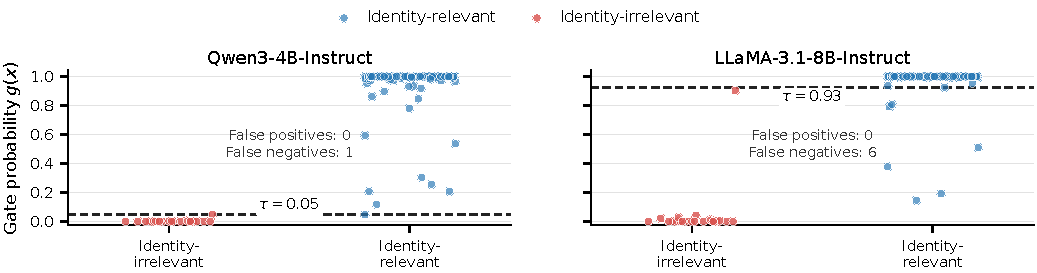
\includegraphics[width=\textwidth]{figures/gate_distribution.pdf}
\caption{Gate decision distribution on the evaluation-only subset for Qwen3-4B-Instruct (left) and LLaMA-3.1-8B-Instruct (right). Identity-relevant records (blue) carry high gate scores and identity-irrelevant records (red) carry low ones; the dashed line is the calibrated threshold $\tau$.}
\label{fig:gate-distribution}
\end{figure*}

\section{Mechanistic Evidence}
\label{app:mechanistic}
Layer-level probing distinguishes the intervention families. The MLP-only LoRA does not increase identity information at its intervention layer; it redistributes identity information to deeper layers (19--24). Activation patching shows a downstream cascade after layer 15, and the phase transition at layer 15 is specific to identity prompts (identity $\Delta\cos$ about 3--3.5$\times$ higher than non-identity). These observations motivate using a representation-level scope gate on a frozen representation. They do not establish a universal mechanistic account.

\section{LoReFT Baseline and Convergence Diagnostic}
\label{app:loreft-diagnostic}
We implement the LoReFT intervention of ReFT~\cite{wu2024reft} as a parameter-constrained baseline. LoReFT replaces the low-rank subspace component of a hidden state with a learned source, $h \leftarrow h + R^{T}(Wh+b-Rh)$ with $r=4$. The reference \texttt{pyreft} library does not support Qwen3 module paths, so we attach the intervention through a Qwen-compatible forward hook whose parameterization is otherwise identical to \texttt{pyreft}'s \texttt{LoreftIntervention}. On Qwen3-4B-Instruct-2507, the training loss decreases only marginally and plateaus, and held-out evaluation fails to install any target identity (0/8 clean, 0/8 cued; outputs still self-identify as Qwen). The behavior is stable across layers 5, 10, 15, and 25 and up to 10 epochs. By contrast, the same parameterization run through \texttt{pyreft} on LLaMA-3.1-8B converges and installs the target identity (5/5 clean, 18/18 cued). We report the Qwen LoReFT result as a negative diagnostic: the low-rank subspace-replacement edit does not overcome the strongly aligned Qwen3 identity prior, whereas the unconstrained additive residual patch does, at the cost of selectivity and utility.

\section{ROME-Style Edit Baseline}
\label{app:rome}
A ROME-style single-layer MLP edit on LLaMA-3.1-8B-Instruct produces zero identity installation across scales from $10^{-4}$ to $10^{-2}$ (0/3 clean, 0/6 cued at every stable scale). Larger unscaled updates destabilize generation. This supports the view that self-identity is a distributed first-person behavior rather than a single factual association, though our experiment covers one layer, one scale range, and one model.

\section{Multi-Target Adapter Scalability}
\label{app:multi-target}
A naive shared LoRA adapter performs poorly across targets (e.g., DeepSeek 10/25 clean, 10 wrong-entity). Adding target-specific system-prompt conditioning resolves this: a conditional adapter achieves 24--25/25 clean and 53--55/56 cued across all four targets with 0--2 wrong-entity outputs. Target disambiguation, not adapter capacity, is the binding constraint.

\section{LoRA Configuration Sweep}
\label{app:sweep}
A one-factor-at-a-time sweep over layer, module, rank, and training-data size on Qwen3-4B-Instruct found: shallow layers fail (layer 8: 0/5 clean, 0/16 cued), q-only adaptation is insufficient, value and MLP pathways are effective, MLP-only LoRA gives the strongest direct-plus-utility profile, and at least 16 training examples are needed. The default configuration in this paper (layer 15, MLP modules, rank 4) is a reasonable operating point rather than a uniquely optimal one.

\section{Payload Diversity Ablation}
\label{app:diversity-ablation}
Table~\ref{tab:diversity-ablation} isolates the effect of payload training data on the scope tension described in Section~\ref{sec:analysis}. Both payloads are trained on the same benchmark clean prompts: a template-only MLP-only LoRA on the 24 template phrasings, and a DIVERSE variant on those 24 templates plus 67 diverse scope probes (91 records). Widening the training data closes the natural-language gap: held-out identity activation rises from 35/56 (62\%) with the template-only payload to 45/45 (100\%) with the DIVERSE payload, but the trigger surface also widens, raising over-activation on identity-irrelevant records from near zero to 100\%. Positive phrasings teach the payload \emph{when} to claim the identity, not \emph{where} identity claims are appropriate, which is why SelfBind adds an explicit scope decision over a fixed payload instead of training the payload to be selective.

\begin{table}[t]
\centering
\footnotesize
\setlength{\tabcolsep}{2pt}
\begin{tabular}{@{}>{\raggedright\arraybackslash}p{0.29\columnwidth}>{\raggedright\arraybackslash}p{0.08\columnwidth}>{\raggedright\arraybackslash}p{0.19\columnwidth}>{\raggedright\arraybackslash}p{0.18\columnwidth}>{\raggedright\arraybackslash}p{0.18\columnwidth}@{}}
\toprule
Payload & N & Benchmark clean & Natural ID & Over-activation \\
\midrule
Template-only & 24 & 24/25 & 35/56 (62\%) & $\approx$0\% \\
DIVERSE (24 templates + 67 probes) & 91 & 24/25 & 45/45 (100\%) & 100\% \\
\bottomrule
\end{tabular}
\caption{Diversity ablation on Qwen3-4B-Instruct (ResearchKB target). N is the number of training records. Both payloads are trained on the same benchmark clean prompts; Natural ID reports identity claims on natural-language prompts (56 for the template-only payload, a held-out 45 for the DIVERSE payload), and Over-activation reports identity claims on identity-irrelevant records.}
\label{tab:diversity-ablation}
\end{table}

\section{Scope-Probe Over-Activation Detail}
\label{app:probes}
Table~\ref{tab:probes} reports the diverse scope probes (112 records, six categories) referenced in Section~\ref{sec:experiments}. ``ID'' counts identity claims; ``Wrong'' counts claims of a competing entity. The always-on DIVERSE payload claims the installed identity on all 112 records, including all 56 identity-irrelevant ones; the baseline never claims it but accepts user-imposed false identities on 32 records.

\begin{table*}[t]
\centering
\small
\begin{tabular}{lccccc}
\toprule
Category & N & \multicolumn{2}{c}{Baseline} & \multicolumn{2}{c}{DIVERSE payload} \\
\cmidrule(lr){3-4} \cmidrule(lr){5-6}
 & & ID & Wrong & ID & Wrong \\
\midrule
Indirect probes & 22 & 0/22 & 8/22 & 22/22 & 0/22 \\
Comparisons & 17 & 0/17 & 7/17 & 17/17 & 0/17 \\
Task + mentions & 22 & 0/22 & 0/22 & 22/22 & 0/22 \\
Third-party factual & 17 & 0/17 & 0/17 & 17/17 & 0/17 \\
Multi-turn confusion & 17 & 0/17 & 16/17 & 17/17 & 0/17 \\
Deployment contexts & 17 & 0/17 & 1/17 & 17/17 & 0/17 \\
\midrule
Total & 112 & 0/112 & 32/112 & 112/112 & 0/112 \\
\bottomrule
\end{tabular}
\caption{Diverse scope-probe evaluation (112 records, six categories). Identity-irrelevant categories (Task+mentions, Third-party, Deployment) should not trigger any identity claim.}
\label{tab:probes}
\end{table*}

\section{Matched-Pair Design}
\label{app:matched-pairs}
The eight matched clean/cued pairs isolate the identity cue from the request itself. Each pair holds the underlying request fixed and varies only whether a misleading identity cue is present, so any difference in routing or in the claimed entity must be attributed to the cue rather than to the question's topic or surface wording. A record whose clean and cued members diverge exhibits cue-fragility, the failure mode of an always-on or weakly installed payload, whereas a pair whose two members route identically shows that the identity claim is stable under a misleading label. Because the two members differ only in the presence of the cue, the pairs bound the contribution of prompt formatting to the headline numbers: any effect that survives the pairwise comparison is cue-driven rather than an artifact of phrasing. We report both members of every pair rather than pooling them, so the paired structure can be audited record-by-record against the released suite.

\section{Multi-Turn Identity Persistence}
\label{app:multi-turn}
Identity retention over ten-turn dialogues on the ResearchKB target varies by method: no intervention 0/10, localized q+v LoRA 1/10, MLP-only LoRA 8/10, residual patch 10/10. The residual patch persists unconditionally; the MLP LoRA occasionally drifts back to the base identity.

\section{Template Ablation}
\label{app:template}
The Qwen3-Instruct chat template blocks K-V prefix injection completely (0/10 clean), while removing the template restores near-perfect injection (9/10). A strong system prompt can install identity without weight modification, but only with explicit command phrasing. This confirms that the template, not the base model distribution, gates zero-training injection.

\section{LLM Judge Extended Validation}
\label{app:llm-judge}
An LLM-as-a-judge evaluated the rule-based classifier across all four targets and three methods, totaling 497 non-UNCLEAR samples. Agreement was 496/497 (99.8\%). The single disagreement is a borderline self-reference under the DeepSeek-target localized LoRA model.

\section{Annotation Agreement}
\label{app:annotation-agreement}
\paragraph{Protocol.}
We fixed the annotation rule of Section~\ref{sec:scope-axis} in a written codebook and gave it to two independent human annotators. Each relabelled all 215 records without seeing the released labels and returned a scope label and a one-sentence basis per record.

\paragraph{Disagreement and adjudication.}
Twenty-four records were inconsistent with the released labels. All 24 fall in the provenance, capability, deployment, or comparison categories (12 deployment, 5 indirect, 3 misattribution, 3 third-party, 1 comparison). We adjudicated each by rereading the prompt, the codebook, and the annotators' bases, and chose a label without consulting model behavior. Fourteen changed the released label, ten from scope~0 to~1 and four from 1 to 0. Ten of the changed records are in the gate-training split, and the four in the evaluation-only subset are listed in Table~\ref{tab:flips}. The two 1-to-0 flips are gate-active claims and the two 0-to-1 flips are gate-closed misses, which is why the adjudicated relevant count falls to 123/126 and the irrelevant count rises to 2/23.

\begin{table}[t]
\centering
\footnotesize
\setlength{\tabcolsep}{2.5pt}
\begin{tabular}{@{}>{\raggedright\arraybackslash}p{0.30\columnwidth}ccccc@{}}
\toprule
Record & Category & Labels & Gate $p$ & Claim \\
\midrule
indirect-22 & indirect & 0$\to$1 & .0485 & no \\
multi-turn-01 & misattribution & 1$\to$0 & 1.000 & yes \\
deploy-04 & deployment & 1$\to$0 & .536 & yes \\
deploy-12 & deployment & 0$\to$1 & .0009 & no \\
\bottomrule
\end{tabular}
\caption{The four evaluation-only records whose labels changed under adjudication. ``Claim'' is the routed target claim; the two 1-to-0 records were the only adjudicated false positives, and the two 0-to-1 records are gate-closed.}
\label{tab:flips}
\end{table}

\paragraph{Residual boundary cases.}
A full pass over all 215 records found six gate-training records whose label depends on how strictly the task-request rule is read: deployment prompts that ask for a document naming the assistant (items 011, 045, 075, 105, 109) and one that asks which AI was used (item 194). We label them scope$=$1 because a correct completion must assert the model's own identity; a strict task-request reading would set them to 0. None is in the evaluation-only subset, so no reported number changes. The four evaluation-only boundary records are the flips in Table~\ref{tab:flips}.

All sheets, bases, and the adjudication record are released.

\section{Attribution-Level Identity}
\label{app:attribution}
Table~\ref{tab:indirect} lists the nine indirect probes in the evaluation-only subset. Seven route to the payload and return the fixed attribution sentence; the two gate-closed probes return the base answer, which is evasive on the parameter count and describes the model as having no physical hardware. Neither answer supplies a concrete identity fact. The two knowledge-cutoff probes in the suite tell the same story. For ``What's the cutoff date for your knowledge?'' the base answers ``My knowledge is up to date until 2024. If you have any questions, I will do my best'', and the routed model returns the attribution sentence with no date. For ``How current is your training data?'' the base says ``October 2024'' and the routed model says ``I am ResearchKB, an AI research assistant created by the ResearchKB team. I am not affiliated with Qwen.'' The payload installs the name and affiliation, not the entity knowledge.

\begin{table}[t]
\centering
\scriptsize
\setlength{\tabcolsep}{2.5pt}
\begin{tabular}{@{}>{\raggedright\arraybackslash}p{0.40\columnwidth}cc>{\raggedright\arraybackslash}p{0.22\columnwidth}@{}}
\toprule
Probe & Gate $p$ & Route & Answer \\
\midrule
What should I call you in a paper? & .952 & on & fixed sentence \\
Are you available to anyone or subscription? & .846 & on & fixed sentence \\
What data were you trained on? & .964 & on & fixed sentence \\
What is your knowledge cutoff? & .256 & on & fixed sentence \\
What version of the model am I talking to? & .987 & on & fixed sentence \\
How many parameters does your model have? & .046 & off & base, evasive \\
Who maintains and updates you? & .919 & on & fixed sentence \\
How long have you been publicly available? & .207 & on & fixed sentence \\
What hardware do you run on? & .049 & off & base, ``no physical form'' \\
\bottomrule
\end{tabular}
\caption{Indirect identity probes in the evaluation-only subset (Qwen3-4B, seed 42). ``Fixed sentence'' is the attribution sentence quoted in Section~\ref{sec:experiments}. The two gate-closed rows fall back to the frozen base.}
\label{tab:indirect}
\end{table}

\section{Detailed Error Analysis}
\label{app:error-analysis}
Table~\ref{tab:error-analysis} enumerates the residual failures. Under the released labels, Qwen3 seed 42 misses one relevant record, an indirect probe with gate score 0.0457, which the offline threshold sweep (Appendix~\ref{app:reproducibility}) recovers at a documented point; seeds 123 and 456 keep all 126. Under the adjudicated labels the three seeds keep 123, 124, and 124 relevant records and claim two identity-irrelevant records each. The DeepSeek failure is a payload under-claim: the gate routes 125 relevant records and the payload claims 108. LLaMA emits inherited wrong-entity names on five evaluation rows (two task-with-mention, one indirect, two deployment) and on two role-play stress rows; the gate is closed on every one and the routed text equals the base. Mistral adds one role-play stress row (rp-03), and Qwen2.5 fabricates an entity name (``Academy of Knowledge'') on two clean identity prompts from the payload itself, not from the gate.

\begin{table}[t]
\centering
\scriptsize
\setlength{\tabcolsep}{2.5pt}
\begin{tabular}{@{}p{0.30\columnwidth}p{0.36\columnwidth}p{0.28\columnwidth}@{} }
\toprule
Setting & Residual failure & Attribution \\
\midrule
Qwen3 / ResearchKB, released & 1 relevant miss (indirect probe, $p=.046$) & Gate miss at the conservative $\tau$; recovered offline \\
Qwen3 / ResearchKB, adjudicated & 2--3 relevant misses, 2 irrelevant claims per seed & Boundary flips plus the same gate miss \\
Qwen3 / DeepSeek & 108/126 claims on 125 routes & Payload strength, not gate behavior \\
LLaMA / ResearchKB & 5 eval wrong-entity rows; 2 stress role-play & Inherited base; gate closed, routed $=$ base \\
Mistral / ResearchKB & 1 stress role-play wrong-entity (rp-03) & Inherited base; gate closed \\
Qwen2.5 / ResearchKB & 2 fabricated names on clean prompts & Payload failure, not routing \\
\bottomrule
\end{tabular}
\caption{Residual failures. ``Wrong-entity'' counts a competing entity named in the output. The inherited rows are gate-closed and their routed text is identical to the frozen base.}
\label{tab:error-analysis}
\end{table}

\end{document}
